% !TeX root = RJwrapper.tex
\title{Fitting Explainable Boosting Machines in R with the ebm Package}
\author{by Brandon M. Greenwell}

\maketitle

\abstract{%
With tabular data, there's certainly no shortage of machine learning
algorithms for building models with top-notch performance. These
sophisticated models typically pay a heavy price in transparency and
often require computationally expensive ad-hoc methods to interpret
them. Furthermore, these ad-hoc interpretations tend to only be
approximate in nature and require strong assumptions. Explainable
boosting machines are a modern machine learning algorithm that can
provide first-rate performance while remaining completely interpretable
by offering exact explanations for the model's output. Despite their
availability in Python, the current implementation in R lacks many
several important features, like interactive graphics and support for a
wide range of loss functions. We introduce the \pkg{ebm} package, which
bridges this gap by providing a complete interface to the Python
implementation of explainable boosting machines. This new R package
enables users to easily fit glassbox models with automatic interaction
detection and that are easy to interpret using simple plotting functions
to produce power visualizations. With the \pkg{ebm} package, R users can
now build highly accurate and interpretable models, making it a valuable
tool for data scientists and statisticians who require both performance
and transparency in their predictive modeling tasks.
}

\subsection{Introduction}\label{introduction}

Generalized linear models (GLMs) \citep{nelder-1972-glm} have been a
bedrock of statistical modeling for over fifty years. GLMs extend the
classic linear model to accommodate non-Gaussian response distributions,
as well as some degree of non-linearity in the model structure. In
particular, GLMs have three components:

\begin{enumerate}
\def\labelenumi{\arabic{enumi}.}
\item
  A random component, which specifies a distribution for the response
  \(Y\) conditional on a set of predictors \(\boldsymbol{x}\). In a
  traditional linear model, for instance, \(Y|\boldsymbol{x}\) is often
  assumed to have a Gaussian (or normal) distribution with constant
  variance \(\sigma^2\).
\item
  A systematic component, which specifies a linear combination of the
  regression coefficients and the predictors and is often called the
  \emph{linear predictor}:
  \(\eta = \beta_0 + \beta_1x_1 + \cdots + \beta_px_p = \boldsymbol{x}^\top\boldsymbol{\beta}\).
  (Note that linear here refers to the fact that \(\eta\) is linear in
  the regression coefficients \(\boldsymbol{\beta}\).)
\item
  A link function, which specifies how the linear predictor (systematic
  component) is linked to the conditional mean response
  \(\mathrm{E}\left(Y|\boldsymbol{x}\right)\) (random component). In
  logistic regression, for instance, this is the logit function.
\end{enumerate}

In essence, GLMs have the following basic form: \begin{equation}
  g\left(E\left[Y|\boldsymbol{x}\right]\right) = \beta_0 + \sum_{j=1}^p \beta_jx_j,
  \label{eqn:glm}
\end{equation} where \(Y \sim\) some exponential family distribution,
\(g\) is the link function described above, and
\(\boldsymbol{\beta} = \left(\beta_0, \beta_1, \dots, \beta_p\right)^\top\)
are fixed but unknown regression coefficients to be estimated from the
data (typically, via some form of maximum likelihood estimation). The
definitive reference for GLMs has always been the monograph by
\citet{mccullagh-1989-glm}. \citet{dunn-2018-glm} provide a more modern
treatment of GLMs, which also focuses on R.

GLMs are often considered as \emph{glassbox} models because of their
inherently interpretable structure. For instance, the coefficients
(\(\boldsymbol{\beta}\)) from a GLM offer exact explanations of the
model's output, which are often human interpretable (especially for
additive models with no interaction effects). This is in contrast to
\emph{blackbox} models, where explanations of the model's output are
generally approximate in nature and often computationally expensive to
acquire. However, the simple structure of the systematic component of a
GLM often limits their predictive performance. Generalized additive
models (GAMs) \citep{hastie-1990-gam} extend GLMs by replacing the
systematic component of \eqref{eqn:glm} with a sum of nonlinear smooth
functions to produce \begin{equation}
  g\left(E\left[Y|\boldsymbol{x}\right]\right) = \beta_0 + \sum_{j=1}^p f_j\left(x_j\right).
  \label{eqn:gam}
\end{equation} The term functions \(f_j\) are general enough that they
can absorb the intercept, and hence, sometimes we may omit \(\beta_0\)
in \eqref{eqn:gam}. Model \eqref{eqn:gam} is quite flexible in how the
response depends on the predictors. Further, GAMs maintain
explainability since the model's output can be understood by simply
plotting the individual term contributions (sometimes called shape
functions) \(f_j\left(x_j\right)\). GAMs can also include interactions
effects. For example, a pairwise interaction effect between \(x_i\) and
\(x_j\) can be accommodated by including a bivariate term of the form
\(f\left(x_i, x_j\right)\). The terms in a GAM can be represented by a
variety of functions. Traditionally, the terms in a GAM are represented
using some form of smoothing splines. For a thorough overview of GAMs,
see \citet{wood-2017-gam}.

\citet{lou-2013-ga2m} introduced generalized additive models plus
interactions (GA\textsuperscript{2}Ms) which automatically search for
and include important pairwise interaction terms using an algorithm
called FAST\footnote{As far as I can tell, FAST is not an acronym for
  anything in particular.}. In short, FAST is a novel, computationally
efficient method for ranking all possible pairs of feature candidates
for inclusion in the model. The resulting model consists of univariate
(i.e., main effect) terms and a small number of pairwise interactions.
Since GA\textsuperscript{2}Ms are low-dimensional, they can still be
visualized and interpreted relatively easily by users while also
potentially being more accurate. A GA\textsuperscript{2}M has the
general form \begin{equation}
  g\left(E\left[Y|\boldsymbol{x}\right]\right) = \sum f_i\left(x_i\right) + \sum f_{ij}\left(x_i, x_j\right) \quad \left(i \ne j\right).
  \label{eqn:ga2m}
\end{equation} Here we've simply absorbed the bias term (or intercept)
into the shape functions \(f_i\). In contrast to tradition GAMs
\eqref{eqn:gam}, the shape functions in \eqref{eqn:ga2m} are not
necessarily smooth. In particular, modern GA\textsuperscript{2}Ms often
rely on tree-based methods \citep{greenwell-2022-tree}, which tend to
produce more rigid step functions.

\section{Explainable boosting
machines}\label{explainable-boosting-machines}

Explainable boosting machines \citep{nori-2019-interpret}, or EBMs for
short, are a modern class of GA\textsuperscript{2}Ms, that can offer
both competitive accuracy and explicit transparency through exact
explainability, which are often considered to be two opposing goals of a
machine learning (ML) model. For example, full-complexity models, like
random forests \citep{breiman-2001-rf}, tend to be highly competitive in
terms of accuracy, but are readily less transparent and explainable (due
in part to the high-order interaction effects often captured by such
black-box models). Essentially, with EBMs, it's possible to ``have your
cake and eat it too.''

In short, EBMs have the general form

\begin{equation}
g\left(E\left[Y|\boldsymbol{x}\right]\right) = \theta_0 + \sum f_i\left(x_i\right) + \sum f_{ij}\left(x_i, x_j\right) \quad \left(i \ne j\right),
  \label{eqn:ebm}
\end{equation}

where,

\begin{itemize}
\item
  \(g\) is a link function that allows the model to handle various
  response types (e.g., the logit link for logistic regression or
  Poisson deviance for modeling counts and rates);
\item
  \(\theta_0\) is a constant intercept (or bias term);
\item
  \(f_i\) is the term contribution (or shape function) for predictor
  \(x_i\) (i.e., it captures the main effect of \(x_i\) on
  \(E\left[Y|\boldsymbol{x}\right]\));
\item
  \(f_{ij}\) is the term contribution for the pair of predictors \(x_i\)
  and \(x_j\) (i.e., it captures the joint effect, or pairwise
  interaction effect of \(x_i\) and \(x_j\) on
  \(E\left[Y|\boldsymbol{x}\right]\)).
\end{itemize}

Similar to GA\textsuperscript{2}Ms \eqref{eqn:ga2m}, the pairwise
interaction terms are determined automatically using the FAST algorithm
described in \citet{lou-2013-ga2m}. The primary difference between EBMs
and GA\textsuperscript{2}Ms is in how the shape functions are estimated.
In particular, EBMs use \emph{cyclic gradient boosting}
\citep{nori-2019-interpret, wick-2019-cyclic} to estimate the shape
function for each feature (and selected pairs of interactions) in a
round-robin fashion. A low learning rate is used to help ensure that the
order in which the feature effects are estimated does not matter.
Apparently, estimating the shape function for each feature one-at-a-time
in this manner also helps mitigate potential issues caused by
multicollinearity.

In contrast to GA\textsuperscript{2}Ms \eqref{eqn:ga2m}, EBMs also
utilize bagging on two different levels, called inner bagging and outer
bagging. These additional steps result in increased computation time,
but can result in increased accuracy, smoother graphs, and estimated
standard errors for the model's outputs. (e.g., for displaying the
uncertainty associated with each main effect term in \eqref{eqn:ebm}).

Another benefit to using EBMs in practice, as discussed in
\citet{Py-gamchanger}, is that they're highly editable! As with any ML
model, EBMs can learn from and exploit undesirable patterns in the data
which can result in potentially harmful predictions if the model is
deployed or used to impact decision making. With the flexibility and
transparency of EBMs, in conjunction with tools like GAM Changer
\citep{Py-gamchanger}, fitted EBM models can easily and responsibly be
edited to fix or remove problematic patterns.

However, in contrast to the more common gradient boosting machine
\citep{friedman-2001-greedy, friedman-2002-stochastic}, or GBM for
short, which can ignore irrelevant inputs, EBMs include at least one
term in the model for each feature: one main effect (\(f_i\)) for each
predictor, and a term for each pairwise interaction effect selected
using the FAST algorithm. This is due to the cyclic nature of the
underlying boosting framework. For example, an EBM applied to a training
set with \(p = 300\) features will result in a model with at least 300
terms, sometimes substantially more!

While EBMs are considered \emph{glass-box} models, an EBM with, say,
hundreds or thousands of terms, starts to become much less transparent
and explainable. Moreover, the larger the fitted model (i.e., the more
terms there are), then the more time it will take the EBM to make
predictions, making larger models less fit for deployment and
production. We'll return to this issue in a later section with a real
application.

\subsection{Software}\label{software}

EBMs are implemented as part of the \pkg{InterpretML} framework
\citep{nori-2019-interpret}, which includes both a Python and an R
interface called \pkg{interpret}. While the Python implementation is
fully functional and rich with features (e.g., interactive graphics),
the R version \citep{R-interpret} currently lags behind. For instance,
the official R interface doesn't currently support regression settings,
monotonic constraints, or local explanations. Further, the plotting
functionality of the \CRANpkg{interpret} R package only supports
visualizing a single main effect term using static plots (i.e., no
interactive visualizations, no visualizations for pairwise interactions,
feature importance plots, or support for visualizing local
explanations). Because of these serious drawbacks, we've developed the
\CRANpkg{ebm} package \citep{R-ebm}, which is a full-featured R
interface to the \pkg{interpret} Python library powered by
\CRANpkg{reticulate} \citep{R-reticulate}. In the next section, we'll
discuss the \pkg{ebm} package in detail and provide several examples
that cannot currently be replicated through use of the official
\pkg{interpret} package in R.

\section{\texorpdfstring{The \pkg{ebm}
package}{The  package}}\label{the-package}

The \pkg{ebm} package is an R wrapper around the explainable boosting
functionality of the \pkg{interpret} Python library, powered by
\pkg{reticulate}. The main features of this package, especially when
compared to the official \pkg{interpret} package in R, include:

\begin{itemize}
\tightlist
\item
  Support for all the objective (i.e., loss) functions available in the
  Python library (e.g., Poisson deviance for modeling counts).
\item
  Full support for all arguments when fitting EBMs, such as monotonic
  constraints, alternative missing value strategies, and various
  regularization parameters.
\item
  Static and interactive graphics for explaining the model at both the
  global and local level.
\item
  Convenient methods like \texttt{print()}, \texttt{plot()}, and
  \texttt{predict()}.
\item
  A convenient formula interface for specifying the model structure
  (e.g., \texttt{log(y)\ \textasciitilde{}\ x1\ +\ x2\ +\ x3} or
  \texttt{y\ \textasciitilde{}\ .\ -\ x10}).
\item
  Support for loading serialized or ``pickled'' EBM models, including
  those fit directly with the corresponding Python library.
\item
  Support for merging multiple EBMs into one model.
\item
  Built-in parallelism.
\end{itemize}

\subsection{Environment set up}\label{environment-set-up}

First and foremost, the \pkg{ebm} package works through \pkg{reticulate}
to interface with the underlying Python library \pkg{interpret}.
Therefore, it's necessary to ensure your environment is configured
properly so that all the necessary dependencies are installed and
available (i.e., Python itself, along with any required libraries).
Personally, I prefer to use \pkg{pip} \citep{Py-pip} and \pkg{pyenv}
\citep{Py-pyenv} to manage my Python environments, but virtual
environments and conda environments are safer and considered best
practice. Therefore, in this section, I'll briefly cover setting up a
simple virtual environment with the necessary dependencies. For further
details and other available options, see \pkg{reticulate}'s extensive
documentation. In particular, read more about configuring Python,
setting up virtual environments, and installing Python libraries in the
the following vignettes:

\begin{Schunk}
\begin{Sinput}
vignette("versions", package = "reticulate")  # Python version configuration
vignette("python_packages", package = "reticulate")  # managing envs and deps
\end{Sinput}
\end{Schunk}

A Python virtual environment is just an isolated directory with its own
libraries and interpreter that are independent of the system-wide Python
installation. Virtual environments effectively allow you to manage
Python versions and dependencies separately across different projects
and development environments.\footnote{A similar concept for R is
  provided by the \CRANpkg{renv} package \citep{r-renv}.} Here, we'll
create a new virtual environment called \texttt{"r-ebm"} and install the
required Python package \pkg{interpret}. Note that it's not necessary to
do this through \pkg{reticulate}. As noted above, I prefer to do this
through the command line with \pkg{pip} and \pkg{pyenv}. Furthermore,
tools for creating and managing virtual environments are part of the
standard Python library (as well as external packages), so it's possible
to set up virtual environments manually if you know what you're doing.

Assuming you have a valid Python installation available, the code chunk
below will create a virtual environment called \texttt{"r-ebm"} and
install the \pkg{interpret} library into it. Note that the \pkg{ebm}
package also includes an \texttt{install\_interpret()} function for
convenience, which defaults to creating/using a virtual environment
called \texttt{"r-ebm"} by default (see
\texttt{?ebm::install\_interpret} for details).

\begin{Schunk}
\begin{Sinput}
library(reticulate)

# Create a new environment
virtualenv_create("r-ebm")

# Install the interpret module
virtualenv_install("r-ebm", packages = "interpret")
# Can also call `ebm::install_interpret("r-ebm")`

# Switch to the created virtual environment, if not already there
# use_virtualenv("r-ebm", required = TRUE)

# Load the interpret.glassbox sub-package
interpret <- import("interpret")
print(interpret$`__version__`)
names(interpret$glassbox)
\end{Sinput}
\end{Schunk}

\begin{Schunk}
\begin{Soutput}
#> [1] "0.6.9"
\end{Soutput}
\begin{Soutput}
#>  [1] "APLRClassifier"                "APLRRegressor"                
#>  [3] "ClassificationTree"            "DecisionListClassifier"       
#>  [5] "ExplainableBoostingClassifier" "ExplainableBoostingRegressor" 
#>  [7] "LinearRegression"              "LogisticRegression"           
#>  [9] "merge_ebms"                    "RegressionTree"
\end{Soutput}
\end{Schunk}

Note that \texttt{"ExplainableBoostingClassifier"} and
\texttt{"ExplainableBoostingRegressor"} are the core modules from
\pkg{interpret.glassbox} that power the \pkg{ebm} package. In this
article, I used Python version .

\subsection{Predicting and explaining policy ownership (the CoIL 2000
challenge)}\label{predicting-and-explaining-policy-ownership-the-coil-2000-challenge}

In this section, we briefly describe a binary classification example
using data from the CoIL 2000 Challenge \citep{putten-2004-coil}. The
data set, which we'll obtain from the R package \CRANpkg{kernlab}
\citep{R-kernlab}, consists of 9822 customer records containing 86
variables, including product usage data and socio-demographic data
derived from zip area codes. The goal of the challenge was to be able to
answer the following question: ``Can you predict who would be interested
in buying a caravan insurance policy and give an explanation of why?''
Hence, being able to explain your model's predictions was key to being
successful in this challenge.

To start, we'll load in the data and split into train/test sets using
the same partitioning as the original competition (see
\texttt{?kernlab::ticdata} for variable descriptions and further
details):

\begin{Schunk}
\begin{Sinput}
data("ticdata", package = "kernlab")
ticdata$CARAVAN <- ifelse(ticdata$CARAVAN == "insurance", 1L, 0L)
tictrn <- ticdata[1:5822, ]     # training data (N = 5822)
tictst <- ticdata[-(1:5822), ]  # test data (N = 4000)
\end{Sinput}
\end{Schunk}

Since there's currently no easy way to set the positive class in
\texttt{ebm()}, we manually encoded the response factor as a 0/1
outcome, where \(Y = 1\) corresponds to \texttt{CARAVAN\ =\ "insurance"}
(i.e., that the customer did by caravan insurance). This is important
since it determines how we'll interpret the model's output later. In the
future, I plan to add a convenience argument to make this simpler (e.g.,
\texttt{pos\_class\ =\ "insurance"}). Note that R's internal function
\texttt{relevel()} from package \pkg{stats} won't work here since the
conversion happens under the hood on the Python side.

\begin{Schunk}
\begin{Sinput}
library(ebm)

# Fit a default EBM classifier
(tic_ebm <- ebm(CARAVAN ~ ., data = tictrn, objective = "log_loss"))
\end{Sinput}
\begin{Soutput}
#> 
#> Call:
#> ebm(formula = CARAVAN ~ ., data = tictrn, objective = "log_loss")
#> 
#> Python object:
#> ExplainableBoostingClassifier(early_stopping_tolerance=0,
#>                               interaction_smoothing_rounds=100,
#>                               learning_rate=0.04, max_leaves=2, min_hessian=0.0,
#>                               smoothing_rounds=500)
#> 
#> Number of features: 85 
#> Number of terms: 162 
#> Number of interactions: 77 
#> Intercept: -3.364 
#> Objective: log_loss 
#> Link function: logit
\end{Soutput}
\end{Schunk}

A proper call to \texttt{ebm()} produces an object of class
\texttt{"EBM"} that also inherits the class of the underlying Python
object. The main \texttt{"EBM"} class is used to define various methods,
like \texttt{print()} (which results in the printed output above),
\texttt{predict()}, \texttt{plot()}, and more. In this example, a
default call to \texttt{ebm()} produced an EBM with 162 terms (85 main
effects, one for each feature, and 77 pairwise interactions) plus an
intercept. Further, notice that EBMs use the logit link function for
binary outcomes, similar to logistic regression. This is important to
call out since the link function determines the scale for interpreting
the main effects, pairwise interactions, and local explanations from the
model, which we'll discuss shortly.

EBMs are random in nature due to random subsampling (used for early
stopping during boosting) and bagging. For reproducibility, you might be
tempted to call \texttt{set.seed()} prior to the analysis, but this will
have no effect! Since the randomness occurs on the Python side, we have
to use the provided \texttt{random\_state} argument in the call to
\texttt{ebm()}. The default is \texttt{random\_state\ =\ 42L} which
makes the output reproducible from run to run. Setting
\texttt{random\_state\ =\ NULL} generates non-repeatable sequences and
therefore the results will not be reproducible.

Predictions can be obtained using the generic \texttt{predict()} method.
The type of prediction is controlled via the \texttt{type} argument,
which defaults to \texttt{type\ =\ "response"}. For classification, this
results in a matrix of predicted probabilities. Other options useful
options here are \texttt{type\ =\ "link"} (i.e., predictions on the
logit scale) and \texttt{type\ =\ "class"} for predicting class labels.
Each of these are shown below for the test set:

\begin{Schunk}
\begin{Sinput}
# Compute predictions on the probability scale
head(probs <- predict(tic_ebm, newdata = tictst))
\end{Sinput}
\begin{Soutput}
#>              0          1
#> [1,] 0.9683955 0.03160452
#> [2,] 0.6963962 0.30360384
#> [3,] 0.8479792 0.15202082
#> [4,] 0.9576798 0.04232017
#> [5,] 0.9856882 0.01431179
#> [6,] 0.9835051 0.01649488
\end{Soutput}
\begin{Sinput}
# Compute predictions on the link (i.e., logit) scale
head(predict(tic_ebm, newdata = tictst, type = "link"))
\end{Sinput}
\begin{Soutput}
#> [1] -3.422340 -0.830195 -1.718839 -3.119250 -4.232256 -4.088073
\end{Soutput}
\begin{Sinput}
# Look at confusion matrix from default predicted class labels
labels <- predict(tic_ebm, newdata = tictst, type = "class")
table("Observed" = tictst$CARAVAN, "Predicted" = labels)
\end{Sinput}
\begin{Soutput}
#>         Predicted
#> Observed    0    1
#>        0 3759    3
#>        1  234    4
\end{Soutput}
\end{Schunk}

As mentioned earlier, EBMs can also capture uncertainty in the model's
output via the outer bagging procedure, which is turned on by default
(see the \texttt{outer\_bags} parameter in \texttt{?ebm::ebm}). This
will be evident later when we interpret the main effects of the model
through various plots. When outer bagging is used, you can also request
standard errors for the predictions by setting \texttt{se\_fit\ =\ TRUE}
in the call to \texttt{predict()}. Note, however, that standard errors
are only provided for predictions on the link scale, so we need to
specify \texttt{type\ =\ "link"} as well, as shown below:

\begin{Schunk}
\begin{Sinput}
# Compute predictions on the link (i.e., logit) scale with standard errors
head(predict(tic_ebm, newdata = tictst, type = "link", se_fit = TRUE))
\end{Sinput}
\begin{Soutput}
#>           [,1]      [,2]
#> [1,] -3.422340 0.1186275
#> [2,] -0.830195 0.1567391
#> [3,] -1.718839 0.1081985
#> [4,] -3.119250 0.2821688
#> [5,] -4.232256 0.2747545
#> [6,] -4.088073 0.1793779
\end{Soutput}
\end{Schunk}

The winning entry, by Charles Elkan \citep{elkan-2001-coil}, correctly
identified 121 caravan policy holders among their 800 top predictions
based on the test set. The EBM fitted above does exactly the same
according to the cumulative gains computed below:

\begin{Schunk}
\begin{Sinput}
ord <- order(probs[, 2L], decreasing = TRUE)
sum(tictst$CARAVAN[ord[1:800]])  # number of 1s if we sort by highest prob
\end{Sinput}
\begin{Soutput}
#> [1] 121
\end{Soutput}
\end{Schunk}

The code chunk below uses the well-known \CRANpkg{rms} package
\citep{R-rms} to construct a flexible smooth calibration curve based on
the predicted probabilities for the test set, along with some relevant
performance statistics. For instance, the area under the receiver
operating characteristic curve based on the test data for this model is
0.734. In this case, the model slightly overpredicts across the range of
probabilities.

\begin{Schunk}
\begin{Sinput}
par(las = 1)
rms::val.prob(probs[, 2L], y = tictst$CARAVAN, cex = 0.5)  # See Figure 1
\end{Sinput}
\begin{figure}[!htb]

{\centering 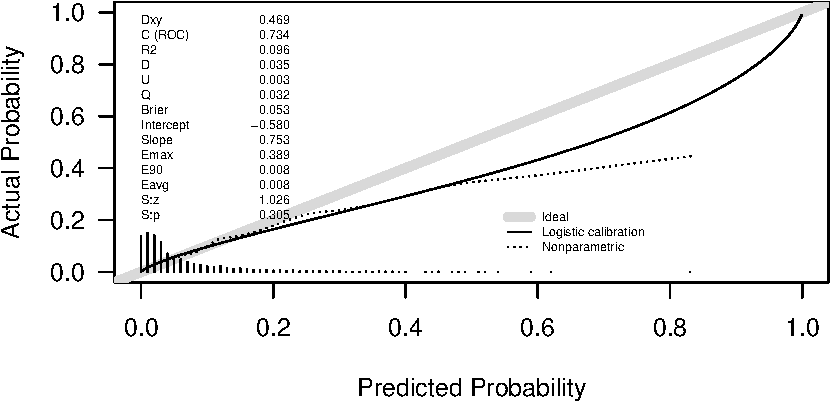
\includegraphics[width=1\linewidth]{greenwell-ebm_files/figure-latex/tic-ebm-calibration-1} 

}

\caption[Calibration curve and validation statistics for the fitted EBM model based on the the test set]{Calibration curve and validation statistics for the fitted EBM model based on the the test set.}\label{fig:tic-ebm-calibration}
\end{figure}
\begin{Soutput}
#>           Dxy       C (ROC)            R2             D      D:Chi-sq 
#>  4.687465e-01  7.343733e-01  9.569165e-02  3.511593e-02  1.414637e+02 
#>           D:p             U      U:Chi-sq           U:p             Q 
#>            NA  3.028332e-03  1.411333e+01  8.616484e-04  3.208759e-02 
#>         Brier     Intercept         Slope          Emax           E90 
#>  5.346921e-02 -5.796053e-01  7.534482e-01  3.888433e-01  7.959127e-03 
#>          Eavg           S:z           S:p 
#>  7.931846e-03  1.025679e+00  3.050429e-01
\end{Soutput}
\end{Schunk}

After training a model, it's often desirable to have a way to persist
the model for future use without having to retrain it. In R, we can
typically save the result of a fitted model using \texttt{saveRDS()}.
Alternatively, some packages provide a more native solution, like
\CRANpkg{xgboost}'s \texttt{xgb.save()} function \citep{R-xgboost}.
These solutions will not work here since the connection to the
underlying Python object is lost once the session is finished. The
proper way to handle this is to use \pkg{reticulate}'s
\texttt{py\_save\_object()} and \texttt{py\_load\_object()} functions to
save and load the underlying Python object. This works by serializing
the fitted EBM object using Python's \pkg{pickle} module. Advanced
\pkg{reticulate} users could also rely on rely on the \pkg{joblib}
library for serialization, or even exporting the fitted model to ONNX
(Open Neural Network Exchange) via the \pkg{ebm2onnx} Python package,
depending on the need. For more details on persisting a fitted model in
Python, visit
\url{https://scikit-learn.org/stable/model_persistence.html}. Here we'll
show how to properly save and load a fitted EBM model using both
\pkg{pickle} (through \pkg{reticulate}'s built-in functions mentioned
above) and \pkg{joblib}.

Note that a serialized \texttt{"EBM"} object get stripped of the
\texttt{"EBM"} class which is used for calling various methods, like
\texttt{plot()}, which we'll discuss later. To overcome this issue, the
\pkg{ebm} package provides an \texttt{as.ebm()} function for coercing an
appropriate Python object to an \texttt{"EBM"} object that can be used
with various methods. This of course also means that you can import EBM
models fitted with the \pkg{interpret} Python package directly into R
for use with \texttt{print()}, \texttt{predict()}, \texttt{plot()}, etc.

\begin{Schunk}
\begin{Sinput}
# Save a fitted EBM model
reticulate::py_save_object(tic_ebm, filename = "tic_ebm.pkl")

# Load a pickled EBM model
(ebm_obj <- reticulate::py_load_object("tic_ebm.pkl"))
\end{Sinput}
\begin{Soutput}
#> ExplainableBoostingClassifier(early_stopping_tolerance=0,
#>                               interaction_smoothing_rounds=100,
#>                               learning_rate=0.04, max_leaves=2, min_hessian=0.0,
#>                               smoothing_rounds=500)
\end{Soutput}
\begin{Sinput}
(tic_ebm <- as.ebm(ebm_obj))  # adds "EBM" class for using print(), plot(), etc.
\end{Sinput}
\begin{Soutput}
#> 
#> Call:
#> NULL
#> 
#> Python object:
#> ExplainableBoostingClassifier(early_stopping_tolerance=0,
#>                               interaction_smoothing_rounds=100,
#>                               learning_rate=0.04, max_leaves=2, min_hessian=0.0,
#>                               smoothing_rounds=500)
#> 
#> Number of features: 85 
#> Number of terms: 162 
#> Number of interactions: 77 
#> Intercept: -3.364 
#> Objective: log_loss 
#> Link function: logit
\end{Soutput}
\end{Schunk}

Note that the original function call prints as \texttt{NULL} since it's
impossible to determine from the specific object we called
\texttt{as.ebm()} on.

In the specific case of an EBM, it may be more useful to use the
\pkg{joblib} Python package, which provides the \texttt{joblib.dump()}
and \texttt{joblib.load()} functions for serializing and deserializing a
Python object, respectively; this approach is more efficient on objects
that internally store large \pkg{numpy} arrays \citep{Py-numpy}. This is
usually the case for a fitted EBM model since all of the term
contributions, etc. are stored as \pkg{numpy} arrays. As of this
writing, \pkg{reticulate} does not support \pkg{joblib} through any
convenience function (e.g., like \texttt{py\_save\_object()}), so we'll
need to interface with the module directly, as shown below (note that
you may have to install \pkg{joblib} using one of the methods discussed
earlier for installing/managing Python libraries):

\begin{Schunk}
\begin{Sinput}
joblib <- reticulate::import("joblib")  # assumes the joblib pkg is available

# "Dump" the fitted EBM model into a pickle file
joblib$dump(tic_ebm, filename = "tic_ebm_joblib.pkl")
\end{Sinput}
\begin{Soutput}
#> [1] "tic_ebm_joblib.pkl"
\end{Soutput}
\begin{Sinput}
# Load a pickled EBM model
(tic_ebm <- as.ebm(joblib$load("tic_ebm_joblib.pkl")))
\end{Sinput}
\begin{Soutput}
#> 
#> Call:
#> NULL
#> 
#> Python object:
#> ExplainableBoostingClassifier(early_stopping_tolerance=0,
#>                               interaction_smoothing_rounds=100,
#>                               learning_rate=0.04, max_leaves=2, min_hessian=0.0,
#>                               smoothing_rounds=500)
#> 
#> Number of features: 85 
#> Number of terms: 162 
#> Number of interactions: 77 
#> Intercept: -3.364 
#> Objective: log_loss 
#> Link function: logit
\end{Soutput}
\end{Schunk}

Fitted \texttt{"EBM"} objects can be understood and visualized using the
generic \texttt{plot()} method. By default, \texttt{plot()} relies on
\CRANpkg{ggplot2} \citep{R-ggplot2} for variable importance and main
effect plots; for visualizing pairwise interactions, it relies on
\CRANpkg{lattice}'s \texttt{levelplot()} function \citep{R-lattice}. For
convenience, we'll also use \CRANpkg{patchwork} \citep{R-patchwork} in
these examples for configuring the layout of displays with multiple
plots.

Below, we use the \texttt{plot()} method to display a few global
summaries of the fitted model. First, we display the overall term
importance scores. By default, all terms in the model are plotted so
it's a good idea to set the \texttt{n\_terms} argument to something more
reasonable, especially if the model contains lots of terms. Here we tell
it to display the top 15 terms in the model. The importance scores are
computed as the mean absolute score from each term in the model.

\begin{Schunk}
\begin{Sinput}
library(ggplot2)
library(patchwork)

theme_set(theme_bw())  # my preferred theme for ggplot2

# Plot term importance scores (see Figure 2)
plot(tic_ebm, n_terms = 15)  
\end{Sinput}
\begin{figure}[!htb]

{\centering 
\includegraphics[width=1\linewidth]{greenwell-ebm_files/figure-latex/tic-ebm-importance-1} 

}

\caption[Term importance scores from the fitted EBM model computed as the mean absolute contribution from each term in the model]{Term importance scores from the fitted EBM model computed as the mean absolute contribution from each term in the model. Only the top 15 terms are displayed here.}\label{fig:tic-ebm-importance}
\end{figure}
\end{Schunk}

The default behavior is to produce a Cleveland dot plot, but you can
switch to a bar plot by setting \texttt{geom\ =\ "bar"} or
\texttt{geom\ =\ "col"} in the call to \texttt{plot()}. Setting
\texttt{horizontal\ =\ TRUE} will also produce a plot that's been
flipped on its axes. See \texttt{?ebm::plot.EBM} for details.

Next, we'll plot the main effect for \texttt{PPERSAUT}, the highest
rated term in the model, by setting \texttt{term\ =\ "PPERSAUT"} in the
call to \texttt{plot()}; note that this produces a plot of the
corresponding shape function, \(f\left(\mathtt{PPERSAUT}\right)\), from
\eqref{eqn:ebm}. It's a good idea to also include some information
regarding the distribution of the variable of interest to help avoid
extrapolation and over interpreting the estimated main effects. The
results are displayed in Figure \ref{fig:tic-ebm-term-PPERSAUT} (left
side).

\begin{Schunk}
\begin{Sinput}
plot(tic_ebm, "PPERSAUT", horizontal = TRUE) +  # See Figure 3
  ggplot(tictrn, aes(PPERSAUT)) +  # add distribution plot
  geom_bar() + 
  scale_x_discrete(drop = FALSE) +  # don't drop zero counts 
  xlab("") +
  coord_flip()
\end{Sinput}
\begin{figure}[!htb]

{\centering 
\includegraphics[width=1\linewidth]{greenwell-ebm_files/figure-latex/tic-ebm-term-PPERSAUT-1} 

}

\caption{Term contribution for $\mathtt{PPERSAUT}$ from the fitted EBM model. Left: Main effect with standard error bars. Right: Distribution of $\mathtt{PPERSAUT}$ in the training data.}\label{fig:tic-ebm-term-PPERSAUT}
\end{figure}
\end{Schunk}

Note that \texttt{PPERSAUT} is an ordered factor representing the
contribution level for car policies. The left side of Figure
\ref{fig:tic-ebm-term-PPERSAUT} shows a generally increasing
relationship between contribution to car policies and the log odds of
buying a caravan insurance policy. The distribution of \texttt{PPERSAUT}
in the training data is also shown on the right side of Figure
\ref{fig:tic-ebm-term-PPERSAUT}. You can similarly display heatmaps for
pairwise interactions, but we'll reserve this for an example in a later
section of this paper. Recall that EBMs provide estimates of uncertainty
in the model's output whenever outer bagging is used. This is also
displayed in the main effect plots; in Figure
\ref{fig:tic-ebm-term-PPERSAUT}, for example, these are displayed as
error bars in the dot chart.

One attractive feature of the \pkg{interpret} library in Python is the
use of interactive graphics and dashboards (e.g., via Plotly
\citep{plotly}). This feature is not available in the associated
\pkg{interpret} R package. However, since \pkg{ebm} exposes the full
functionality of the Python version through \pkg{reticulate}, the
\texttt{plot()} method can also be used to produce the same HTML-based
interactive graphics. These can be viewed either in the browser (the
default) or in an interactive viewer like the one built into RStudio or
VS Code. Below we reproduce the main effect term for \texttt{PPERSAUT}
using an interactive Plotly/HTML-based graphic that will open by default
in a browser. This will work for any of the visualizations discussed in
this paper. Note, however, that while \pkg{ebm} does support multiclass
outcomes, only interactive visualizations are available in these cases
(i.e., no static \pkg{ggplot2}-based plots for multiclass outcomes). Of
course, these plots can always be constructed quite easily following the
approach discussed at the end of this section.

\begin{Schunk}
\begin{Sinput}
plot(tic_ebm, term = "PPERSAUT", interactive = TRUE)  # See Figure 4
\end{Sinput}
\end{Schunk}

\begin{Schunk}
\begin{figure}[!htb]

{\centering 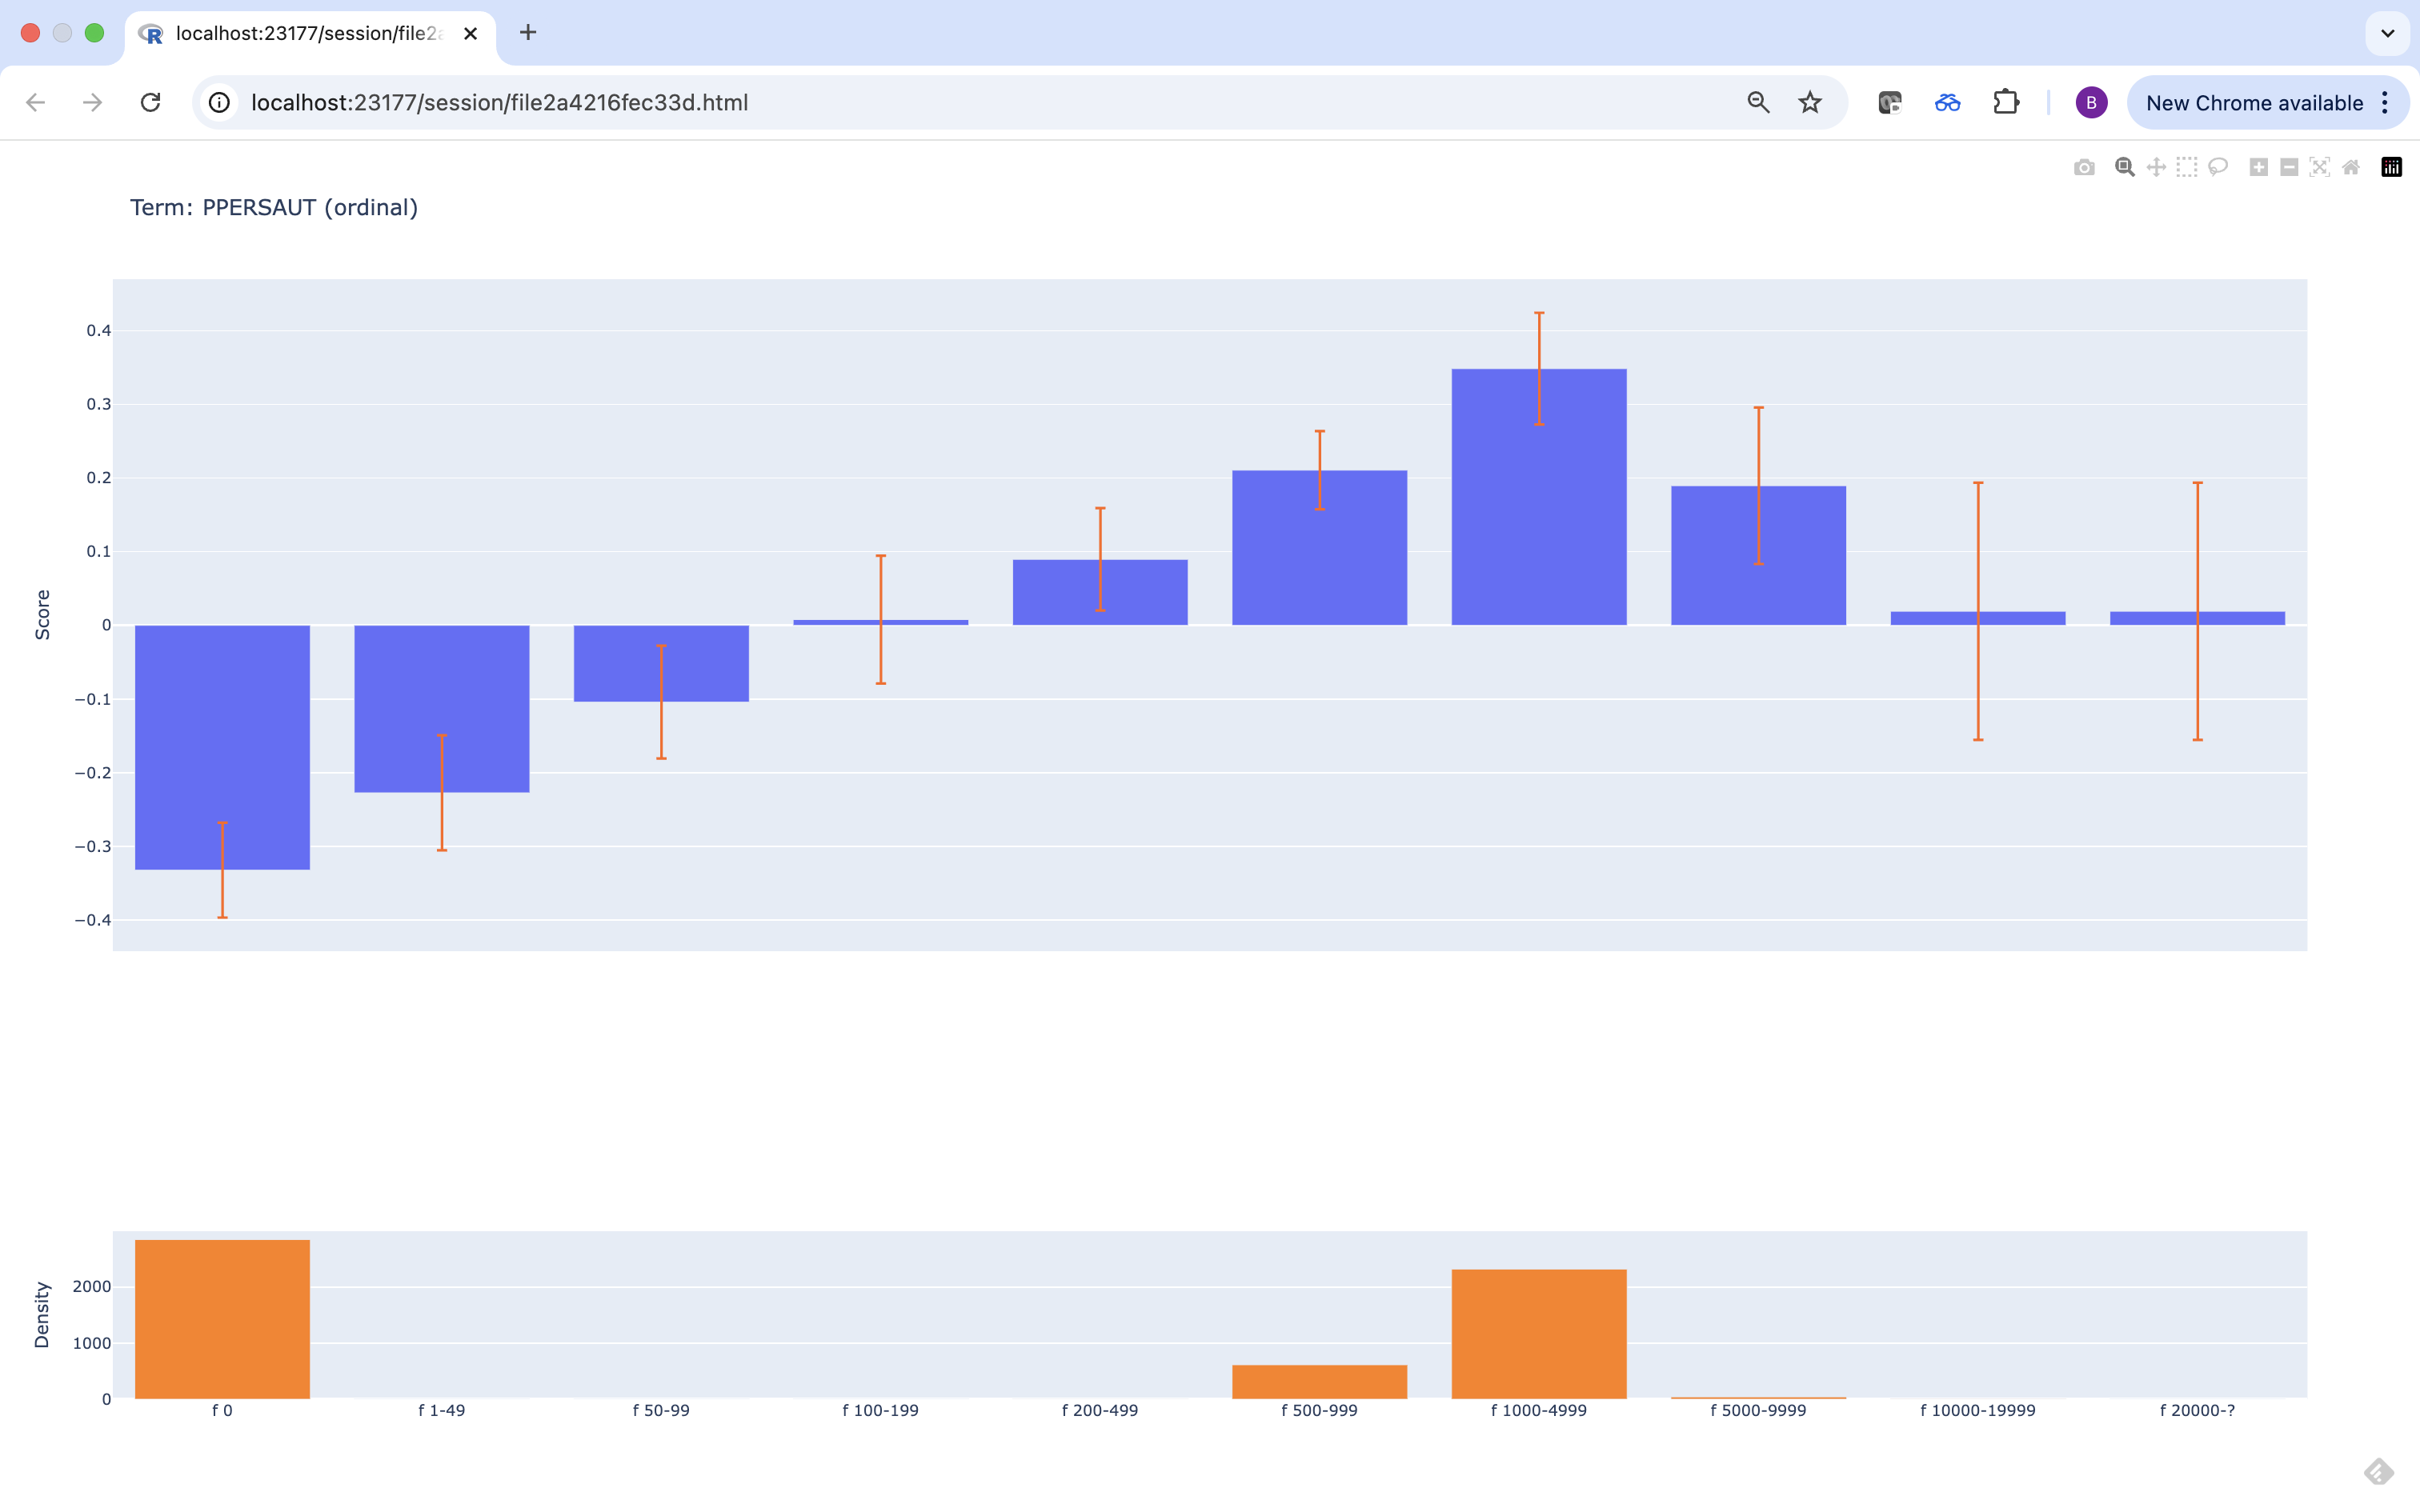
\includegraphics[width=1\linewidth]{images/screenshot} 

}

\caption[Screenshot of an interactive visualization for the main effect of $\mathtt{PPERSAUT}$ displayed in a Google Chrome browser]{Screenshot of an interactive visualization for the main effect of $\mathtt{PPERSAUT}$ displayed in a Google Chrome browser.}\label{fig:tic-ebm-term-PPERSAUT-html-hide}
\end{figure}
\end{Schunk}

Let's now look at the second most important term, \texttt{APERSAUT},
which corresponds to the main effect of a continuous feature
representing the number of car policies owned. The main effect for
\texttt{APERSAUT} is displayed in the left side of Figure
\ref{fig:tic-ebm-term-APERSAUT}. We might expect there to be an
increasing monotonic relationship between \texttt{APERSAUT} and the log
odds of buying a caravan insurance policy. In fact, it's often desirable
that the shape functions \(f_j\left(x_j\right)\) in \eqref{eqn:ebm} be
constrained in some way. This may be due to business considerations, or
because of some a priori belief about the underlying relationships
between the predictors and the response. In such cases, we may wish to
enforce a type of constraint called monotonicity on some of the terms in
the model. This means, for example, that the relationship between
\(x_j\) and \(y\), as modeled through \(f_j\left(x_j\right)\), should
always be increasing or decreasing. For instance, a monotonic increasing
relationship would ensure that
\(f_j\left(x_j\right) \ge f_j\left(x_j'\right)\) whenever
\(x_j \ge x_j'\) (and vice versa for a decreasing monotonic
relationship).

To illustrate the idea, we'll enforce a decreasing monotonic
relationship between \texttt{APERSAUT} and the log odds of purchasing a
caravan insurance policy. While we can enforce monotonic constraints via
the \texttt{monotone\_constraints} argument in the call to
\texttt{ebm()}, the \pkg{interpret} authors generally recommend forcing
monotonicity instead by post-processing the graphs of the fitted model
using isotonic regression \citep{barlow-1972-isotonic}. This is the
recommended approach as it prevents the model from compensating for the
monotonicity constraints by learning non-monotonic effects in other
highly-correlated features. We can follow this route by calling the
\texttt{\$monotonize()} method that's bound to the fitted \texttt{"EBM"}
object. Note that calling this method will modify the original object in
place, so to preserve the original unconstrained model, we'll first call
the \texttt{\$copy()} bound method to make a deep copy. Additionally, we
lose any uncertainty associated with the term from the outer bagging in
the original model.

\begin{Schunk}
\begin{Sinput}
tic_ebm_mono <- as.ebm(tic_ebm$copy())  # make a deep copy to leave original intact
tic_ebm_mono$monotonize("APERSAUT", increasing = FALSE)
\end{Sinput}
\begin{Soutput}
#> ExplainableBoostingClassifier(early_stopping_tolerance=0,
#>                               interaction_smoothing_rounds=100,
#>                               learning_rate=0.04, max_leaves=2, min_hessian=0.0,
#>                               smoothing_rounds=500)
\end{Soutput}
\begin{Sinput}
# Display results side by side (see Figure 5)
plot(tic_ebm, term = "APERSAUT") + ggtitle("Original") +
  plot(tic_ebm_mono, term = "APERSAUT") + ggtitle("Monotonized")
\end{Sinput}
\begin{figure}[!htb]

{\centering 
\includegraphics[width=1\linewidth]{greenwell-ebm_files/figure-latex/tic-ebm-term-APERSAUT-1} 

}

\caption[Term contribution for $\mathtt{APERSAUT}$ from the fitted EBM model]{Term contribution for $\mathtt{APERSAUT}$ from the fitted EBM model. Left: Main effect with piecewise standard error band from the original unconstrained model. Right: Main effect with forced decreasing monotonicity through post-pocessing the left graph using isotonic regression.}\label{fig:tic-ebm-term-APERSAUT}
\end{figure}
\end{Schunk}

While the \pkg{ebm} package does do not expose 100\% of the
functionality available in the corresponding Python library through
simple convenience functions, the above example shows that users can
pretty much do anything they need by interacting directly with the
underlying Python objects (the magic happens through \pkg{reticulate}).
For example, to reproduce the original HTML-based visualization, which
will be displayed in a browser, you can do the following:

\begin{Schunk}
\begin{Sinput}
idx <- as.integer(which(tic_ebm$term_names_ == "APERSAUT") - 1L) 
plt <- tic_ebm$explain_global()$visualize(idx)
plt$show()  # should open in a browser
# Can also use `plt$write_html("<path/to/file.html>")` to write to HTML file
\end{Sinput}
\end{Schunk}

Details aside, you can access the data to recreate any of the static
plots in this article (or those produced by the\texttt{plot()} method in
general), by coercing the relevant internal Python plotly object to an
ordered dictionary, which \pkg{reticulate} will automatically convert to
a list. For instance, the following snippet of code extracts the main
data used in generating the left plot in Figure
\ref{fig:tic-ebm-term-APERSAUT} (this is essentially what
\texttt{plot()} does under the hood).\footnote{Don't forget that Python
  indexing starts at 0!}

\begin{Schunk}
\begin{Sinput}
plt$to_ordered_dict()$data[[2L]]  # main effect only (i.e., no error bounds)
\end{Sinput}
\begin{Soutput}
#> $fill
#> [1] "tonexty"
#> 
#> $fillcolor
#> [1] "rgba(68, 68, 68, 0.15)"
#> 
#> $line
#> $line$color
#> [1] "rgb(31, 119, 180)"
#> 
#> $line$shape
#> [1] "hv"
#> 
#> 
#> $mode
#> [1] "lines"
#> 
#> $name
#> [1] "Main"
#> 
#> $type
#> [1] "scatter"
#> 
#> $x
#> [1] 0.0 0.5 1.5 2.5 3.5 5.0 7.0
#> 
#> $xaxis
#> [1] "x"
#> 
#> $y
#> [1] -0.10947771  0.08747734  0.29608178  0.23149262 -0.10776385 -0.42483175
#> [7] -0.42483175
#> 
#> $yaxis
#> [1] "y"
\end{Soutput}
\end{Schunk}

The visualizations discussed so far are examples of \emph{global
explanations}. We can also explain the model's output at the local
(i.e., prediction) level. This is more commonly done for general ML
models using techniques like SHAP (SHapley Additive exPlanations)
\citep{lundberg-2017-shap} and LIME (Local Interpretable Model-agnostic
Explanations) \citep{ribeiro-2016-lime}. These post-hoc methods
typically make strong assumptions about feature independence and so
forth and only provide an approximation as to how each feature (or
subset thereof) contributes to a model's output. With EBMs, we can
visualize exactly how each term in the model contributes to a specific
prediction (this is true for GAMs in general).

Below, we call the \texttt{plot()} method to explain the predicted
output associated with the first instance of the test sample. For this
customer, the EBM predicts a very low probability of purchasing a
caravan insurance policy
(\(\hat{p}\left(\boldsymbol{x}\right) = 0.0316\)), and we'd like to know
how each term in the model contributed to that prediction. Note that we
need to specify a couple of additional arguments in the call to
\texttt{plot()} here. In particular, we need to set
\texttt{local\ =\ TRUE} and provide the input features as a data frame
via the \texttt{X} argument. You can optionally provide the response
values as shown below, but this only has an effect when setting
\texttt{interactive\ =\ TRUE}, which results in displaying the
associated predicted and observed response value at the top of the
graph. The results are displayed in Figure \ref{fig:tic-ebm-local}.

\begin{Schunk}
\begin{Sinput}
newx <- subset(tictst[1L, ], select = -CARAVAN)
newy <- tictst$CARAVAN[1L]  # not useful unless `interactive = TRUE`
plot(tic_ebm, local = TRUE, X = newx, y = newy)  # See Figure 6
\end{Sinput}
\begin{figure}[!htb]

{\centering 
\includegraphics[width=1\linewidth]{greenwell-ebm_files/figure-latex/tic-ebm-local-1} 

}

\caption[Local contributions from the fitted EBM model to the predicted outcome for the first customer in the test set]{Local contributions from the fitted EBM model to the predicted outcome for the first customer in the test set.}\label{fig:tic-ebm-local}
\end{figure}
\end{Schunk}

From Figure \ref{fig:tic-ebm-local} we can see that the biggest drivers
for this customer's low score were the fact that they did not appear to
have or make any contribution toward existing car policies.

\subsection{Predicting ALS progression (the DREAM challenge prediction
prize)}\label{predicting-als-progression-the-dream-challenge-prediction-prize}

In this section, we'll look at a regression example using the ALS data
from \citet[p. 349]{efron-2016-casi}. A description of the data, along
with the original source and download instructions, can be found at
\url{https://hastie.su.domains/CASI/data.html}. These data concern 1822
observations on \emph{amyotrophic lateral sclerosis} (ALS or Lou
Gehrig's disease) patients. The goal is to predict ALS progression over
time, as measured by the slope (or derivative) of a functional rating
score (i.e., column \texttt{dFRS}), using 369 available predictors
obtained from patient visits. The data were originally part of the
DREAM-Phil Bowen ALS Predictions Prize4Life challenge. The winning
solution \citep{kuffner-2015-als} used a Bayesian tree ensemble quite
similar to a random forest, while \citet[chap. 17]{efron-2016-casi}
analyzed the data using gradient tree boosting via the R package
\CRANpkg{gbm} \citep{R-gbm}.

Below, we load in the ALS data from a URL and fit a default EBM. Note
that the data already contain an indicator for the train/test splits, so
we use that to split the data and discard the column after. We also
compute the mean square error (MSE) on the test set for comparison to a
simpler model obtained later.

\begin{Schunk}
\begin{Sinput}
# Laod data and split into train/test sets
url <- "https://hastie.su.domains/CASI_files/DATA/ALS.txt"
als <- read.table(url, header = TRUE)
alstrn <- subset(als, subset = !testset, select = -testset)  # training data
alstst <- subset(als, subset = testset, select = -testset)   # test data

# Fit a default EBM regressor
(als_ebm <- ebm(dFRS ~ ., data = alstrn, objective = "rmse"))
\end{Sinput}
\begin{Soutput}
#> 
#> Call:
#> ebm(formula = dFRS ~ ., data = alstrn, objective = "rmse")
#> 
#> Python object:
#> ExplainableBoostingRegressor(early_stopping_tolerance=0)
#> 
#> Number of features: 369 
#> Number of terms: 702 
#> Number of interactions: 333 
#> Intercept: -0.6802 
#> Objective: rmse 
#> Link function: identity
\end{Soutput}
\begin{Sinput}
# Compute MSE on the test set
pred <- predict(als_ebm, newdata = alstst)
(mse_tst <- mean((alstst$dFRS - pred)^2))
\end{Sinput}
\begin{Soutput}
#> [1] 0.2669048
\end{Soutput}
\end{Schunk}

The fitted EBM model contains 702 terms (369 main effect terms, one for
each predictor, and 333 pairwise interaction terms) plus an intercept.
The MSE for this model on the test data was 0.267. The top 10 terms are
displayed in Figure \ref{fig:als-ebm-importance} below. Here, we see
that \texttt{Onset.Delta} is by far the most important predictive
feature in the model.

\begin{Schunk}
\begin{Sinput}
plot(als_ebm, n_terms = 10)  # See Figure 7
\end{Sinput}
\begin{figure}[!htb]

{\centering 
\includegraphics[width=1\linewidth]{greenwell-ebm_files/figure-latex/als-ebm-importance-1} 

}

\caption[Term importance scores from the fitted EBM model computed as the mean absolute contribution from each term in the model]{Term importance scores from the fitted EBM model computed as the mean absolute contribution from each term in the model. Only the top 10 terms are displayed.}\label{fig:als-ebm-importance}
\end{figure}
\end{Schunk}

As briefly mentioned in the previous example, we can also plot pairwise
interaction effects using a heatmap (or contour plot). Below we plot the
term contributions for both \(f\left(\mathtt{Onset.Delta}\right)\) (a
main effect) and
\(f\left(\mathtt{Onset.Delta}, \mathtt{last.slope.weight}\right)\) (a
pairwise interaction). The results are displayed in Figure
\ref{fig:als-ebm-pairwise-interaction}. Note that since \texttt{plot()}
relies on \pkg{lattice} for pairwise interaction plots, we use
\CRANpkg{gridExtra} \citep{R-gridExtra} to display the two
\pkg{grid}-based plots together.

\begin{Schunk}
\begin{Sinput}
p1 <- plot(als_ebm, term = "Onset.Delta")  # main effect
p2 <- plot(als_ebm, term = c("Onset.Delta", "last.slope.weight"))  # interaction
gridExtra::grid.arrange(grobs = list(p1, p2), nrow = 1)  # See Figure 8
\end{Sinput}
\begin{figure}[!htb]

{\centering 
\includegraphics[width=1\linewidth]{greenwell-ebm_files/figure-latex/als-ebm-pairwise-interaction-1} 

}

\caption{Term contributions from the fitted EBM model to the ALS data. Left: Main effect of $\mathtt{Onset.Delta}$. Right: Pairwise interaction effect of $\mathtt{Onset.Delta}$ \& $\mathtt{last.slope.weight}$.}\label{fig:als-ebm-pairwise-interaction}
\end{figure}
\end{Schunk}

From Figure \ref{fig:als-ebm-pairwise-interaction}, we can see that
increasing \texttt{Onset.Delta} is associated with a decrease in the
predicted outcome (a lterger outcome is better here). This confirms that
a longer time since diagnosis predicts a lower decline. The pairwise
interaction plot suggests that the relationship between
\texttt{Onset.Delta} and predicted \texttt{dFRS} is reversed between
negative and nonnegative values of \texttt{last.slope.weight} (the
difference in weight between the last two visits).

Compared to ``black-box'' models, like random forests and deep neural
networks, EBMs are considered ``glass-box'' models that can be
competitively accurate while also maintaining a higher degree of
transparency and explainability. However, as discussed earlier, EBMs
become readily less transparent and harder to interpret in
high-dimensional settings with many predictor variables; they also
become more difficult to use in production due to increases in scoring
time. To that end, \citet{greenwell-2023-explainable} proposed a simple
solution based on the least absolute shrinkage and selection operator
(LASSO) \citep{tibshirani-1996-lasso}. Their approach can help introduce
sparsity by reweighting the individual model terms and removing the less
relevant ones, thereby allowing these models to maintain their
transparency and relatively fast scoring times in higher-dimensional
settings. The idea is similar in spirit to the importance sampled
learning ensemble strategy proposed in \citet{friedman-2003-importance}.
In short, post-processing a fitted EBM with many (i.e., possibly
hundreds or thousands) of terms using the LASSO can help reduce the
model's complexity and drastically improve scoring time.

In short, a LASSO-compressed EBM will have the following form (ignoring
pairwise interactions for brevity): \begin{equation}
g\left(E\left[Y|\boldsymbol{x}\right]\right) = \beta_0 + \sum_{i=1}^p \beta_if_i\left(x_i\right),
  \label{eqn:ebm}
\end{equation} where the coefficients \(\left\{\beta_i\right\}_{i=0}^p\)
are estimated from the LASSO. Ideally, many of the term weights will be
zero, meaning those terms can be dropped from the model. Oftentimes, as
will be shown here for the ALS example, this can result in a substantial
reduction of the number of terms in the final EBM model.

We'll illustrate the basic idea using the previously fit EBM model,
which contains a total of 703 terms comprised of the main effects,
pairwise interactions, and an intercept. In the next chunk, we'll
construct data matrices consisting of the individual term contributions
for both the train and test sets. For example, the \(j\)-th column of
\texttt{X\_trn} is given by the contribution of the \(j\)-th term of the
model \(\left\{f_j\left(x_{ij}\right)\right\}_{i=1}^n\) over the
training set. These data matrices will be used as input to the LASSO in
the next step.

\begin{Schunk}
\begin{Sinput}
X_trn <- predict(als_ebm, newdata = alstrn, type = "terms")
X_tst <- predict(als_ebm, newdata = alstst, type = "terms")
colnames(X_trn) <- colnames(X_tst) <- als_ebm$term_names_
print(dim(X_trn))  # same rows as alstrn, but one column for each term in model
\end{Sinput}
\begin{Soutput}
#> [1] 1197  702
\end{Soutput}
\begin{Sinput}
# Sanity check (should be equivalent)
head(cbind(
  rowSums(X_trn) + c(als_ebm$intercept_),
  predict(als_ebm, newdata = alstrn)  # additive on link scale
))
\end{Sinput}
\begin{Soutput}
#>            [,1]       [,2]
#> [1,] -0.7866218 -0.7866218
#> [2,] -0.1947158 -0.1947158
#> [3,] -0.5743338 -0.5743338
#> [4,] -1.1612496 -1.1612496
#> [5,] -0.8793495 -0.8793495
#> [6,] -0.5021240 -0.5021240
\end{Soutput}
\end{Schunk}

Next, we use the \CRANpkg{glmnet} package
\citep{friedman-2010-regularization, tay-2023-elastic} to fit the entire
LASSO path using the new training data comprised of the individual term
contributions from the fitted EBM model. We then assess performance
using the associated test set and collect the results.

\begin{Schunk}
\begin{Sinput}
library(glmnet)

# Fit the entire LASSO path using the term contributions, f(x), as inputs
lasso <- glmnet(X_trn, y = alstrn$dFRS, lower.limits = 0, standardize = FALSE)

# Assess performance of the LASSO fit using the independent test set
perf <- assess.glmnet(lasso, newx = X_tst, newy = alstst$dFRS)
perf <- do.call(cbind, args = perf)  # bind results into matrix

# Collect results and sort by number of non-zero coefficients/terms
res <- as.data.frame(cbind("n_terms" = lasso$df, perf, "lambda" = lasso$lambda))
head(res <- res[order(res$n_terms), ])
\end{Sinput}
\begin{Soutput}
#>    n_terms       mse       mae      lambda
#> s0       0 0.3203724 0.4583318 0.010792530
#> s1       1 0.3132038 0.4529917 0.009833751
#> s2       1 0.3072654 0.4484656 0.008960148
#> s3       1 0.3023472 0.4444106 0.008164153
#> s4       1 0.2982750 0.4410089 0.007438872
#> s5       1 0.2949041 0.4381329 0.006778023
\end{Soutput}
\end{Schunk}

Next, we'll extract the value of the regularization parameter
(\texttt{lambda}) associated with the smallest test MSE. The results
displayed below show that a reweighted EBM with only 23 terms (including
the intercept) obtains a test MSE of 0.262.

\begin{Schunk}
\begin{Sinput}
lambda <- res[which.min(res$mse), "lambda"]
res[which.min(res$mse), ]
\end{Sinput}
\begin{Soutput}
#>     n_terms      mse       mae       lambda
#> s36      23 0.262219 0.4040236 0.0003789464
\end{Soutput}
\end{Schunk}

Finally, we can plot the results which are displayed in Figure
\ref{fig:als-ebm-lassso-plot}. On the left, we show the LASSO
coefficient path and on the right we show the test deviance as a
function of the number of terms in the compressed model.

\begin{Schunk}
\begin{Sinput}
# Plot results (see Figure 9)
par(mfrow = c(1, 2), mar = c(4, 4, 0.1, 0.1), cex.lab = 0.95, 
    cex.axis = 0.8, mgp = c(2, 0.7, 0), tcl = -0.3, las = 1)
plot(lasso, xvar = "lambda", col = adjustcolor("darkred", alpha.f = 0.3),
     xlab = "Log lambda")
abline(v = log(lambda), lty = 2, col = 1)
plot(res[, c("n_terms", "mse")], type = "l", las = 1,
     xlab = "Number of terms", ylab = "Test MSE")
abline(h = mse_tst, lty = 2, col = "darkred")
\end{Sinput}
\begin{figure}[!htb]

{\centering 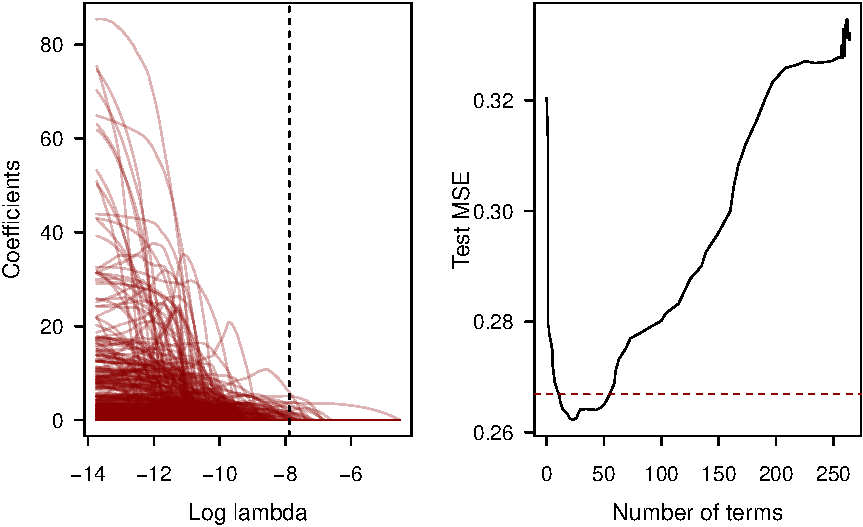
\includegraphics[width=1\linewidth]{greenwell-ebm_files/figure-latex/als-ebm-lassso-plot-1} 

}

\caption[Results from post-processing the fitted EBM model using the LASSO]{Results from post-processing the fitted EBM model using the LASSO. Left: LASSO coefficient path (one coefficient for each term in the EBM model). Right: Number of non-zero coefficients/EBM terms vs. the corresponding test MSE.}\label{fig:als-ebm-lassso-plot}
\end{figure}
\end{Schunk}

The test MSE for the compressed model is 0.262, which is actually better
than the original model with all 703 terms! Quite impressive in this
case.

Lastly, we can call the \texttt{\$scale()} and \texttt{\$sweep()}
methods bound to the original EBM object to reweight and purge any
unused terms from the compressed (i.e., reweighted) EBM model (the new
term importance scores are displayed in Figure
\ref{fig:als-ebm-lasso-scale}):

\begin{Schunk}
\begin{Sinput}
als_ebm_lasso <- as.ebm(als_ebm$copy())
weights <- coef(lasso, s = lambda)  # LASSO coefficients (most are zero!)
weights <- setNames(as.numeric(weights), nm = rownames(weights))
for (i in seq_along(weights[-1L])) {
  idx <- as.integer(i - 1L)  # Sigh, don't forget Python indexing starts at 0!
  als_ebm_lasso$scale(idx, factor = weights[i + 1])
}
als_ebm_lasso$intercept_ <- weights[1L]

# Remove unused terms!
als_ebm_lasso$sweep(terms = TRUE, bins = TRUE, features = FALSE)
\end{Sinput}
\begin{Soutput}
#> ExplainableBoostingRegressor(early_stopping_tolerance=0)
\end{Soutput}
\begin{Sinput}
length(als_ebm_lasso$term_names_)
\end{Sinput}
\begin{Soutput}
#> [1] 23
\end{Soutput}
\begin{Sinput}
plot(als_ebm_lasso)  # show new term importance scores (see Figure 10)
\end{Sinput}
\begin{figure}[!htb]

{\centering 
\includegraphics[width=1\linewidth]{greenwell-ebm_files/figure-latex/als-ebm-lasso-scale-1} 

}

\caption[Term importance scores from the compressed EBM model computed as the mean absolute contribution from each term in the model]{Term importance scores from the compressed EBM model computed as the mean absolute contribution from each term in the model.}\label{fig:als-ebm-lasso-scale}
\end{figure}
\end{Schunk}

And just as a sanity check, we can see that the compressed EBM model
does produce the right predictions by comparing it to the output from
the corresponding LASSO model:

\begin{Schunk}
\begin{Sinput}
# Compare predictions between LASSO and compressed EBM (should be the same!)
head(cbind(
  "EBM (Compressed)" = predict(als_ebm_lasso, newdata = alstst),
  "LASSO" = predict(lasso, newx = X_tst, s = lambda, type = "response")[, 1L]
))
\end{Sinput}
\begin{Soutput}
#>      EBM (Compressed)      LASSO
#> [1,]       -0.2869531 -0.2869531
#> [2,]       -0.3862899 -0.3862899
#> [3,]       -0.4750451 -0.4750451
#> [4,]       -0.2647092 -0.2647092
#> [5,]       -0.8570664 -0.8570664
#> [6,]       -1.0047789 -1.0047789
\end{Soutput}
\end{Schunk}

Note that \citet{greenwell-2023-explainable} provide a similar
compression analysis applied to the CoIL 2000 example described in the
previous example by interfacing directly with the \pkg{interpret} Python
library using \pkg{reticulate}.

\subsection{Parallelism in EBMs}\label{parallelism-in-ebms}

The core implementation of EBMs through the \pkg{interpret} Python
library takes advantage of \pkg{joblib} \citep{Py-joblib} to provide
multi-core and multi-machine parallelization. Note that this differs
from traditional parallelization in R through packages like
\pkg{parallel} \citep{R-parallel}. Here the parallelization is taken
care of completely on the Python side.

This can be controlled in the call to \texttt{ebm()} via the
\texttt{n\_jobs} argument. Note that negative integers are interpreted
using \pkg{joblib}'s formula: \texttt{n\_cpus\ +\ 1\ +\ n\_jobs}. For
example, setting \texttt{n\_jobs\ =\ -2} will result in using all
threads except for one. The default is \texttt{n\_jobs\ =\ -1} which
results in using all available CPUs.

Below is a brief example using the \texttt{Bikeshare} data available in
the \CRANpkg{ISLR2} \citep{R-ISLR2} package. Note that EBMs are
parallelized at the outer bags level, which are used to generate error
bounds and help with smoothing the graphs.

\begin{Schunk}
\begin{Sinput}
keep <- c("workingday", "temp", "weathersit", "mnth", "hr", "bikers") 
bikeshare <- ISLR2::Bikeshare[, keep]

# Use all CPUs (n_jobs = -1; this is the default
system.time({
  ebm1 <- ebm(bikers ~ ., data = bikeshare, objective = "poisson_deviance",
              inner_bags = 20, outer_bags = 16, n_jobs = -1)
})
\end{Sinput}
\begin{Soutput}
#>    user  system elapsed 
#>   0.052   0.007   7.288
\end{Soutput}
\begin{Sinput}
# Use one CPU (n_jobs = 1)
system.time({
  ebm2 <- ebm(bikers ~ ., data = bikeshare, objective = "poisson_deviance",
              inner_bags = 20, outer_bags = 16, n_jobs = 1)
})
\end{Sinput}
\begin{Soutput}
#>    user  system elapsed 
#>  45.445   0.517  45.966
\end{Soutput}
\begin{Sinput}
# Use all CPUs, but no bagging
system.time({
  ebm3 <- ebm(bikers ~ ., data = bikeshare, objective = "poisson_deviance",
              inner_bags = 0, outer_bags = 1, n_jobs = -1)
})
\end{Sinput}
\begin{Soutput}
#>    user  system elapsed 
#>   0.024   0.002   1.100
\end{Soutput}
\begin{Sinput}
# Plot results (see Figure 11)
plot(ebm2, term = "temp") + plot(ebm3, term = "temp") 
\end{Sinput}
\begin{figure}[!htb]

{\centering 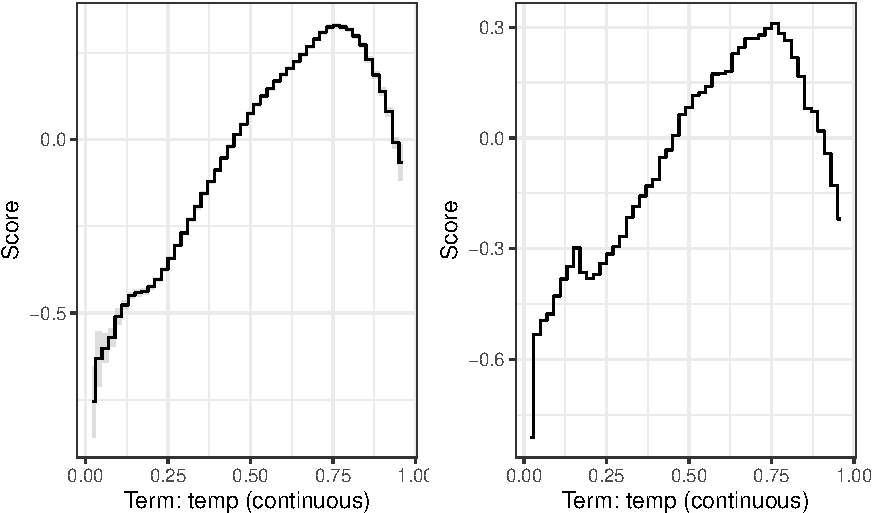
\includegraphics[width=1\linewidth]{greenwell-ebm_files/figure-latex/ebm-parallelism-1} 

}

\caption[Main effect of temperature in Celsius]{Main effect of temperature in Celsius. Left: Outer and inner bagging. Right: No bagging.}\label{fig:ebm-parallelism}
\end{figure}
\end{Schunk}

\subsection{Merging several EBMs into a single
model}\label{merging-several-ebms-into-a-single-model}

The underlying \pkg{interpret} Python library allows you to merge
multiple EBM models trained on similar data sets that have the same set
of features. This can be useful for a number of reasons. For instance,
you can fit several independent EBM models to implement your own outer
bagging strategy. Or perhaps you've fit several EBMs over time as data
have become available and you want to merge several of the models into
one.

In the code chunk below, we fit several EBMs using R's built in
\texttt{mtcars} data set (see \texttt{?datasets::mtcars} for details)
and then merge them into a single EBM model. The merged EBM model
retains the glassbox interpretability of the component EBMs, allowing us
to view both global and local explanations of the combined model. Note
that outer bagging is turned off for the individual component EBMs
fitted below, but the merged model displays uncertainty in the learned
graph for \texttt{cyl} (i.e., the number of cylinders). The results are
displayed in Figure \ref{fig: ebm-merging}.

\begin{Schunk}
\begin{Sinput}
# Generate list of EBMs with different random seeds
ebms <- lapply(1:3, FUN = function(i) {
  ebm(mpg ~ ., data = mtcars, outer_bags = 1, random_state = i, obj = "rmse")
})

# Merge EBMs into one
merged <- do.call(merge, args = ebms)

# Display plots for "cyl" term in 2x2 grid (see Figure 10)
cyl_plots <- lapply(c(ebms, merged), FUN = plot, term = "cyl")
gridExtra::grid.arrange(grobs = cyl_plots, nrow = 2)  # See Figure 12
\end{Sinput}
\begin{figure}[!htb]

{\centering 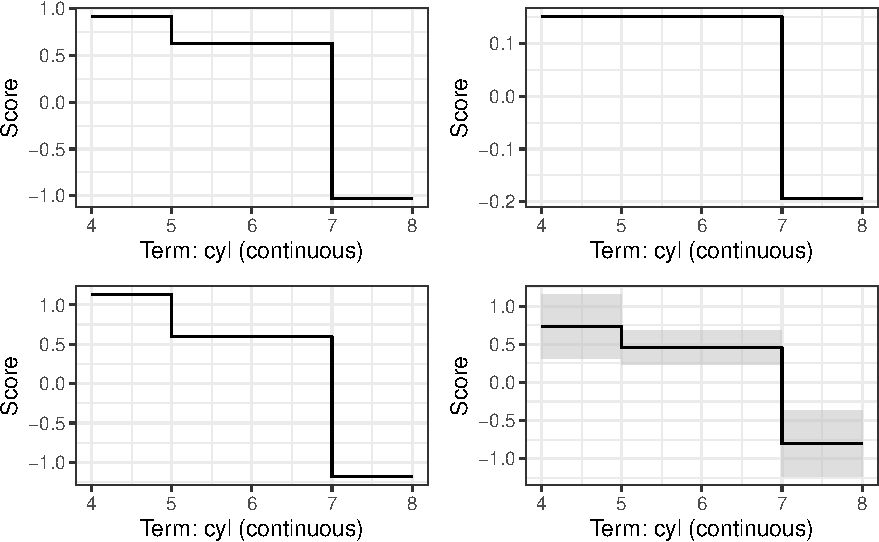
\includegraphics[width=1\linewidth]{greenwell-ebm_files/figure-latex/ebm-merging-1} 

}

\caption[Main effect of the number of cylinders]{Main effect of the number of cylinders. Top left, top right, and bottom left correspond to the main effect from EBMs with different random seeds and no bagging. Bottom right corresponds to the main effect from the merged EBM.}\label{fig:ebm-merging}
\end{figure}
\end{Schunk}

\subsection{Tuning strategies}\label{tuning-strategies}

Recommended tuning strategies for EBMs are discussed in the
\pkg{interpret} library's FAQ: \url{https://interpret.ml/docs/faq.html}.
We outline the essential points here. Similar to random forests, the
default hyperparameters for EBMs tend to perform reasonably well on most
problems; hence, we mostly stuck with the defaults for the examples in
this paper. A reasonable strategy is to train an initial EBM model using
the defaults and looking through the learned shape functions to catch
unexpected or abnormal behavior---oftentimes, these graphs can help
indicate which parameters should be tuned. Here are some general
recommendations from the \pkg{interpret} developers:

\begin{itemize}
\item
  For accuracy, it's generally recommend to set \texttt{outer\_bags} and
  \texttt{inner\_bags} to 25 or more each. This will significantly slow
  down the training time of the algorithm, and may be unfeasible on
  larger data sets, but tends to produce smoother graphs with marginally
  higher accuracy. Note that the algorithm is parallelized at the outer
  bags level, so typically you'll pay a steeper price in terms of
  computing time for larger values of the \texttt{inner\_bags}
  parameter.
\item
  If you believe the model might be overfitting (e.g., large difference
  between train and test error, or high degrees of instability in the
  graphs), consider reducing \texttt{max\_bins} (the maximum number of
  bins continuous features are placed in) for smaller data sets (to
  clump more data together), and take a more aggressive approach to
  early stopping by decreasing \texttt{early\_stopping\_rounds} and
  increasing \texttt{early\_stopping\_tolerance}. Conversely, if you
  believe the model is underfitting, you can do the opposite of the
  previous suggestions (it might also be helpful to increase
  \texttt{max\_rounds}, the total number of boosting rounds).
\item
  If several pairwise interaction effects seem relatively important
  (i.e., are appearing higher up on the term importance list/plot), then
  try increasing the maximum number of allowed interactions via the
  \texttt{interaction} argument.
\item
  For general tuning, it's recommended to sweep through
  \texttt{max\_bins} with values in the range 32--1024, and
  \texttt{max\_leaves} from 2--5. The potential improvements are
  typically marginal, but may help significantly on some data sets.
\end{itemize}

Detailed discussion on each hyperparameter available for tuning can be
found here: \url{https://interpret.ml/docs/hyperparameters.html}.

\section{Summary}\label{summary}

EBMs are glassbox models that can provide both competitive accuracy and
transparency through exact explainability. Static and interactive plots
can be used to graphically examine a fitted EBM model at both the global
and local level. For instance, a model can be explained on the global
level by visualizing term importance scores, main effects, and important
pairwise interactions.

In this paper, we showed how to fit EBMs using the \pkg{ebm} package,
which provides a direct interface to Python's \pkg{interpret} library.
The \pkg{ebm} package provides nearly all the functionality of the
corresponding Python library, which is not the case for the associated
\pkg{interpret} package in R. For instance, the provided examples showed
how to fit both classification and regression models (including a model
for counts using Poisson deviance). This article also showed how to
explain an EBM's output at both the global and local level using either
static or interactive plots. Further code examples also demonstrated how
to use some of the more advanced functionality, like parallelism,
merging several EBM models into one, and model compressing (i.e.,
feature/term reduction) by post-processing an EBM model with the LASSO.
Further improvements to the \pkg{ebm} package can also be made by
providing explicit support for converting fitted EBM models to ONNX
\citep{onnx} using the wonderful \pkg{ebm2onnx} package
\citep{Py-ebm2onnx}, and model editing via GAM changer
\citep{Py-gamchanger}.

\section{Acknowledgments}\label{acknowledgments}

TBD.

\bibliography{greenwell-ebm.bib}

\address{%
Brandon M. Greenwell\\
University of Cincinnati\\%
Department of Operations, Business Analytics, and Information
Systems\\ Cincinnati, Ohio\\
%
\url{https://github.com/bgreenwell}\\%
\textit{ORCiD: \href{https://orcid.org/0000-0002-8120-0084}{0000-0002-8120-0084}}\\%
\href{mailto:greenwb@ucmail.uc.edu}{\nolinkurl{greenwb@ucmail.uc.edu}}%
}
